\documentclass{article}
\usepackage{amsmath, amssymb}
\usepackage{tikz}
\usepackage{geometry}
\usepackage{listings}
\usepackage{xcolor}
\geometry{margin=1in}


\usepackage{pgfplots}
\pgfplotsset{compat=1.18}



\title{Scalar Descent and Fracture Analysis in P3 Space}
\author{Lawrence C. Andrews}
\date{\today}

\definecolor{codegray}{rgb}{0.5,0.5,0.5}
\definecolor{backcolor}{rgb}{0.95,0.95,0.95}

\lstset{
	backgroundcolor=\color{backcolor},
	basicstyle=\ttfamily\small,
	keywordstyle=\color{blue},
	commentstyle=\color{codegray},
	numbers=left,
	numberstyle=\tiny\color{codegray},
	stepnumber=1,
	numbersep=5pt,
	breaklines=true,
	frame=single,
	captionpos=b
}

\begin{document}
	
	\maketitle
	
	\section{Scalar Descent Path with Fracture Persistence}
	
	The following table represents a descent path in P3 space, with fracture annotations and persistence values:
	
	\begin{center}
		\begin{tabular}{|c|c|c|c|c|c|c|}
			\hline
			Step & P3 Input & Reduction Outcome & Fracture ID & Birth T & Death T & Persistence \\
			\hline
			0 & $P_0$ & Canonical & — & — & — & — \\
			1 & $P_0 + \delta_1$ & Slight misalignment & $F_1$ & 0.12 & 0.46 & 0.34 \\
			2 & $P_0 + \delta_2$ & Flip across fold B & $F_2$ & 0.28 & 0.36 & 0.08 \\
			3 & $P_0 + \delta_3$ & Stuck in corner & $F_3$ & 0.05 & 0.67 & 0.62 \\
			\hline
		\end{tabular}
	\end{center}
	
	\section{Simplicial Bin Network with Fracture Connections}
	
	Each vertex represents a scalar bin. Edges represent adjacency relations via reduction or fracture events. Edge labels denote fracture identifiers.
	
	\begin{center}
		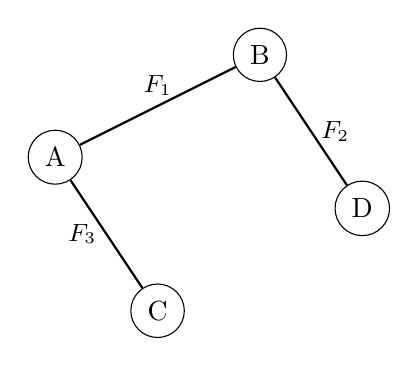
\begin{tikzpicture}[scale=1.3]
			\node (A) at (0,0) [circle,draw] {A};
			\node (B) at (2,1) [circle,draw] {B};
			\node (C) at (1,-1.5) [circle,draw] {C};
			\node (D) at (3,-0.5) [circle,draw] {D};
			
			\draw[thick] (A) -- (B) node[midway,above] {\small $F_1$};
			\draw[thick] (A) -- (C) node[midway,left]  {\small $F_3$};
			\draw[thick] (B) -- (D) node[midway,right] {\small $F_2$};
		\end{tikzpicture}
	\end{center}
	
	\section{Bin Merging Protocol Based on Stability}
	
	This code snippet defines merge conditions based on fracture persistence and signature similarity.
	
	\begin{lstlisting}[language=C++,caption={Bin Merge Criteria Based on Scalar Stability}]
		bool shouldMerge(const ScalarBin& bin1, const ScalarBin& bin2, double persistence) {
			return (persistence < 0.1) &&
			(signatureDistance(bin1.signature, bin2.signature) < 0.05) &&
			(isPermutationInvariant(bin1, bin2));
		}
	\end{lstlisting}
	
	This helps define bin boundaries that reflect stable scalar neighborhoods in fold space.
	
	
		
		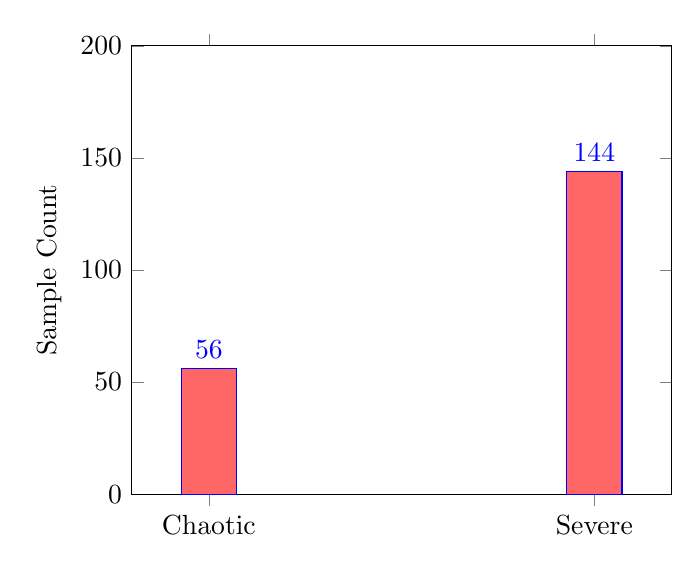
\begin{tikzpicture}
			\begin{axis}[
				ybar,
				bar width=20pt,
				ylabel={Sample Count},
				xtick=data,
				symbolic x coords={Chaotic, Severe},
				xticklabel style={rotate=0},
				ymin=0, ymax=200,
				nodes near coords,
				enlarge x limits=0.2
				]
				\addplot+[fill=red!60] coordinates {(Chaotic,56) (Severe,144)};
			\end{axis}
		\end{tikzpicture}
		
	\end{document}
	
	
\end{document}
